The weak phase \phis is an important parameter of the \BBbarSyst system. It is related to the third
type of CP-Violation mentioned in \secref{Phenomenology}, nameley in the interference between
two decay amplitudes, see \figref{interference}. In the current section the parameter \phis
and its relevance to the search for new particles is introduced. The status of the \phis
measurements concludes the section.

\newcommand{\ffig}{f}
\newcommand{\phimixfig}{\phi_\text{mix}}
\newcommand{\phifig}{\phi_\text{dec}}
\newcommand{\phibarfig}{\kern 0.15em \overline{\kern -0.15em \phi_\text{dec} \kern -0.60em} \kern 0.60em}
\begin{figure}[h]
  \centering
  \resizebox{0.4\textwidth}{!}{\begin{picture}(0,0)%
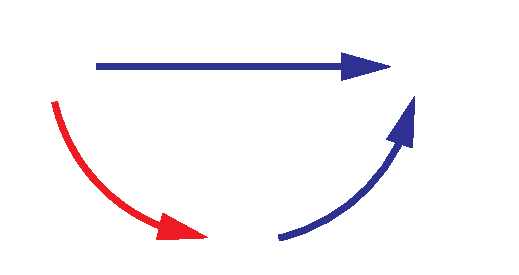
\includegraphics{Figures/Chapter1/decay_CMYK.pdf}%
\end{picture}%
\setlength{\unitlength}{4144sp}%
%
\begingroup\makeatletter\ifx\SetFigFont\undefined%
\gdef\SetFigFont#1#2#3#4#5{%
  \reset@font\fontsize{#1}{#2pt}%
  \fontfamily{#3}\fontseries{#4}\fontshape{#5}%
  \selectfont}%
\fi\endgroup%
\begin{picture}(3939,2094)(2644,-2188)
\put(3286,-736){\makebox(0,0)[rb]{\smash{{\SetFigFont{25}{30.0}{\sfdefault}{\mddefault}{\updefault}{\color[rgb]{0,0,0}$\Bs$}%
}}}}
\put(5761,-736){\makebox(0,0)[lb]{\smash{{\SetFigFont{25}{30.0}{\sfdefault}{\mddefault}{\updefault}{\color[rgb]{0,0,0}$\ffig$}%
}}}}
\put(4501,-421){\makebox(0,0)[b]{\smash{{\SetFigFont{25}{30.0}{\sfdefault}{\mddefault}{\updefault}{\color[rgb]{0,0,1}}%
}}}}
\put(5581,-1771){\makebox(0,0)[lb]{\smash{{\SetFigFont{25}{30.0}{\sfdefault}{\mddefault}{\updefault}{\color[rgb]{0,0,1}}%
}}}}
\put(3331,-1771){\makebox(0,0)[rb]{\smash{{\SetFigFont{25}{30.0}{\sfdefault}{\mddefault}{\updefault}{\color[rgb]{1,0,0}}%
}}}}
\put(4501,-2041){\makebox(0,0)[b]{\smash{{\SetFigFont{25}{30.0}{\sfdefault}{\mddefault}{\updefault}{\color[rgb]{0,0,0}$\Bsb$}%
}}}}
\end{picture}%
}
  \caption{The two interfering decay amplitudes leading to the same final state.
           The phases $\phimixfig$, $\phifig$ correspond to ....
           % This is assuming no CP violation in mixing or CP violation in decay.}
           }
  \label{interference}
\end{figure}

The parameter \phis manifests in the so called $\bquark \rightarrow \cquark\cquarkbar\squark $ transitions, where the
\bquark of the \Bs meson decays into three other quarks. In addtion, the final state of the \Bs meson has to be a CP eigenstate,
which implies that both \Bs and \Bsb can decay into it.

A common parameter that is used to parametrize CP violation in the interference between mixing and decay is shown in \equref{lambda_cpv}.

\begin{equation}
 \lambda_{f} = \frac{q}{p} \frac{\bar{A}_f}{A_f}. % \equiv \left|\lambda_f\right| e^{i\phis}.
\label{lambda_cpv}
\end{equation}

\noindent The ratios $|\qoverp|$ and $|\nicefrac{A_f}{\bar{A}_{f}}|$ are ascociated to the mixing and decay parts of \figref{interference} respectivelly.
Given the so called {\it master equations}{\color{red} ref pdg} for the decay rates of a \Bs and \Bsb
to a final state $f$, the asymmetry due to the interference between mixing and decay\footnote{assuming $|\qoverp|=1$ and $|\nicefrac{A_f}{\bar{A}_{\bar{f}}}| = 1$ consistet with {\color{red} ref for nocpv in mix and decay}.}
is shown in \equref{cpv_interf}

\newcommand{\half}{\frac{1}{2}}
\begin{equation}
  \Acp{\text{inter}}(t) = \frac{ - \Im(\lambda_f) \sin(\Delta m_s t)} {\cosh(\half \Delta\Gamma_s t) - \Re(\lambda_f)\sinh(\half\Delta\Gamma_s t)}.
\label{cpv_interf}
\end{equation}

\noindent It is intreasting to point out that according to \equref{cpv_interf} CP asymmetry can be observed in the interference of decay and mixing
even if no CP-Violation occurs in both the mixing and the decay. Since the CP asymmetry can vanish at a certain point of time or for a given time
\equref{cpv_interf} has to remain time dependent.

\begin{figure}[h]
  \centering
  {\sffamily \input{Figures/Chapter1/tree}}
  \caption{{\color{red} Fix this to look more like \figref{QuarkMixing} and put ckm elements on the vertices}}
  \label{bs2jpsiphi}
\end{figure}

Given a certain final state $f$ \equref{lambda_cpv} can be expresed as a combination of CKM elements and thus obtain an
estimate on $\Im(\lambda_f)$ based on the Standard Model. The typical choise for $f$ is the $\jpsi\phi$ for reasons
explained later in this section. The leading order diagrams for the \BsJpsiPhi decay and the \BBbarSyst mixing are
shown in \figref{bs2jpsiphi} and \figref{bs_box} repsectivelly. From those diagrams the $\qoverp$ and $\nicefrac{A_f}{\bar{A}_{f}}$
can be read as shown in \equref{qoverp}\footnote{Here it has been used {\color{red} equation blah from pdg} } and \equref{af_afbar} repsectivelly.

\begin{equation}
 \frac{q}{p} = \frac{\Vtb^*\Vts}{\Vtb\Vts^*}
\label{qoverp}
\end{equation}

\begin{equation}
 \frac{\bar{A}_{\jpsi\phi}} {A_{\jpsi\phi}} = \frac{\Vcb\Vcs^*}{\Vcb^*\Vcs}
\label{af_afbar}
\end{equation}

\noindent From \equref{qoverp}, \equref{af_afbar} and \equref{lambda_cpv} the imaginary part of $\lambda_{f}$ is now computed in,
\equref{phis_def}\footnote{Based on the fact that for a complex number's argument, $\argu{z}$ it is: $\argu{z^{-1}}=\argu{-z}=\argu{z^*}=-\argu{z}$}.

\begin{align}
 \Im(\lambda_f) =& \sin\parenthesis{ \argu{\frac{\Vtb^*\Vts}{\Vtb\Vts^*}} + \argu{\frac{\Vcb\Vcs^*}{\Vcb^*\Vcs}} } \nonumber \\
                =& \sin\parenthesis{ \argu{\parenthesis{\Vtb^*\Vts}^2}    + \argu{\frac{1}{\parenthesis{\Vcb^*\Vcs}^2}} }
                = \sin\parenthesis{  2 \; \argu{\frac{\Vtb^*\Vts}{\Vcb^*\Vcs}} } \nonumber \\
                =& \sin\parenthesis{-2\betas}
                \equiv \sin\parenthesis{\phis}
 \label{phis_def}
\end{align}

\noindent An additional implication arises from the choice of the $\jpsi\phi$ as the final state.
Specifically due to the fact that the last particles have a non zero spin quantum number, their combined wavefunction
is not a pure cp eigenstate. The eigenvalue($+1$ or $-1$) of the combined wavefunction dependants on the total angular momentum
$l$ of the $\jpsi$ and $\phi$ particles. This dependancy has to be taken into acount in \equref{phis_def} resulting in \equref{phis_jpsiphi_def}

\begin{equation}
 \Im(\lambda_{\jpsi\phi}) = (-1)^l\sin\parenthesis{\phis}
 \label{phis_jpsiphi_def}
\end{equation}


\subsubsection{Measuring \phis}

The parameter \phis has been measuremed by the \lhcb experiment by analysing the decays of \BsJpsiPhi.
The
Pros and cons of the final state
Flavour taging, angular analysis
clean phi resonance, high yield, muons and kaons are good for lhcb


\begin{itemize}
  \item \phis measurement status
  \item Show how do you read phis from the decay time distribution. Show terms in pdf (maybe)
\end{itemize}

\subsubsection{New Physics effects in \phis}
All of the above was asuming tree decays only. But there are penguins as well. blhaaaaaaaaaaaaahhhhhhhhhhhhhhh.
 New particles in the box, new vector boson. Mention some types of models.
